%       Syntax from following sources
%               https://www.sharelatex.com/learn/Sections_and_chapters
%               https://www.sharelatex.com/learn/Table_of_contents
%               http://www.bibtex.org/Using/
%               https://www.economics.utoronto.ca/osborne/latex/BIBTEX.HTM
%               https://www.latex-tutorial.com/tutorials/beginners/latex-bibtex/
%               http://tex.stackexchange.com/questions/205/what-graphics-packages-are-there-for-creating-graphics-in-latex-documents
% 		http://www.emerson.emory.edu/services/latex/latex_132.html

% Main stuff
%\documentclass[a4paper,10pt]{article}
\documentclass[12pt]{report}
%      \usepackage{utathesis}
%

\documentclass{report}
\usepackage[utf8]{inputenc}

%% Math Packages
\usepackage{amssymb}
\usepackage{amsmath}
\usepackage{amsfonts}

%% Date Time Pakcages
\usepackage[USenglish]{babel}
\usepackage[nodayofweek,level]{datetime}
\usepackage[margin=0.5in]{geometry}

%% Formatting Packages
\usepackage{indentfirst}

%% Citation Packages
\usepackage{cite}
\usepackage{hyperref}

%% Tables Packages
\usepackage{array,booktabs,ragged2e}

%% SVG Packages
\usepackage{svg}
%\setsvg{
%	inkscape = inkscape -z -D 
%	% conversion options for svg package, export drawing instead of page
%}

%% Commands Section
%\newcommand{\logentry}[4]{ \selectlanguage{USenglish} \formatdate{#2}{#1}{#3}  & {#4}  \\ \hline}
\newcommand{\cW}[1]{^{W}_{C}{#1}}
\newcommand{\tR}[0]{\ensuremath{^{A}}}
\newcommand{\bR}[0]{\ensuremath{_{A}}}
\newcommand{\tL}[0]{\ensuremath{^{B}}}
\newcommand{\bL}[0]{\ensuremath{_{B}}}
\newcommand{\tT}[0]{\ensuremath{^{\intercal}}}
\newcommand{\rL}[0]{\ensuremath{{\tL\bR}}}
\newcommand{\xL}[0]{\ensuremath{{\tL\mathbf{x}}}}
\newcommand{\xR}[0]{\ensuremath{{\tR\mathbf{x}}}}
\newcommand{\hxL}[0]{\ensuremath{{\tL\tilde{\mathbf{x}}}}}
\newcommand{\hxR}[0]{\ensuremath{{\tR\tilde{\mathbf{x}}}}}
\newcommand{\rLM}[0]{\ensuremath{{\tL\bR}\mathbf{M}}}
\newcommand{\rLR}[0]{\ensuremath{{\tL\bR}\mathbf{R}}}
\newcommand{\rLt}[0]{\ensuremath{{\tL\bR}\mathbf{t}}}
\newcommand{\skewsym}[1]{\ensuremath{\left[#1\right]_{\times}}}
\newcommand{\sR}[0]{\ensuremath{^{A}\mathbb{S}}}
\newcommand{\sL}[0]{\ensuremath{^{B}\mathbb{S}}}
\newcommand{\lR}[0]{\ensuremath{{^{A}l}}}
\newcommand{\lL}[0]{\ensuremath{{^{B}l}}}
%% ColumnTypes Section
\newcolumntype{R}[1]{>{\RaggedLeft\arraybackslash}p{#1}}

\title{Thesis or Article}
\author{JeffGWood@mavs.uta.edu}
\date{\today}

\pdfinfo{%
  /Title    (Thesis or Article)
  /Author   (Jeff Wood)
  /Creator  ()
  /Producer ()
  /Subject  ()
  /Keywords ()
}

\begin{document}
\Huge
\maketitle
\large
\newpage
\tableofcontents
\newpage
%\Huge\center\textbf{Geometric Formulas for \newline Computer Vision \& \newline Computer Graphics}\newline

%\large Written by Jeff Wood in LaTeX environment\newline
%\large Updated 2016/03/06 \newline

%\normalsize
%\flushleft
\chapter{Introduction}
%\begin{flushleft}
\par Through the development of applications such as augmented and virtual reality, object / scene reconstruction and visual effects, the process of generating images from an arbitrary vantage point can be found in a variety of applications. In this Thesis (or Article) I will discuss various methods for Image Creation from an arbitraryvantage point, which can be accomplished by two main methodologies of Geometric Construction and Image Synthesis. While both methods use stereo correspondance of multiple images, they differ in the way information is stored and used.
\par Geometric Construction (GC) contains information about the real-world spatial properties (Coordinates in space, Color), thus viewing results are non-constrained in vantage point. Image Synthesis (IS) relies on image properties (pixel displacement) and is thus viewing results are imited in the possible vantage points.
\newpage

\section*{Symbols and Notation}

\begin{tabular}{R{2cm} p{14cm}}
\toprule
\multicolumn{1}{l}{\textbf{Symbol}} & \textbf{Description} \\
\midrule
$\mathbf{v}$ & \textit{Vectors} in \textit{lowercase} bold\\
$v_a$ & \textit{a}-component of vector $\mathbf{v}$ \\
$\mathbf{M}$ & \textit{Matrices} in \textit{uppercase} bold\\ 
$M_{r,c}$ & Entry in row \textit{r} and column \textit{c} of matrix $\mathbf{M}$\\
$\mathbf{m}_c$ & \textit{Vector} occurring in column \textit{c} of matrix $\mathbf{M}$\\
$\mathbf{x}$ & Generic 3-dimensional spatial coordinate\\
$\mathbf{\tilde{x}}$ & Generic 3-dimensional spatial coordinate (expressed \textit{homogeneously})\\

$\mathbf{y}$ & Generic 2-dimensionals image coordinate\\
$\mathbf{\tilde{y}}$ & Generic 2-dimensional image coordinate (expressed \textit{homogeneously})\\


$\mathbf{u}$ & Pixelized 2-dimensional image coordinate\\
$\mathbf{\tilde{u}}$ & Pixelized 2-dimensional image coordinate (expressed \textit{homogeneously})\\


$^{A}{\mathbf{x}}$ & Generic 3-dimensional spatial coordinate in reference frame \textit{A} \\
$^{A}{\mathbf{\tilde{x}}}$ & Generic 3-dimensional spatial coordinate (expressed \textit{homogeneously}) in reference frame {A} \\
$^{C}_{B}\mathbf{\tilde{M}}$ & Change from of reference frame \textit{B} to reference frame \textit{C}\\
$s$ & Normalizing factor applied to \textit{homogeneous} vector $\mathbf{\tilde{v}}$ such that original $\mathbf{v}=s\cdot\mathbf{\tilde{v}}$ is recovered\\
$^{D}\mathbb{S}$ & Spatial reference frame \textit{D}\\
$\skewsym{\mathbf{x}}$ & Skew-symmetric matrix version of vector $\mathbf{x}$ used as \textit{left}-operand in the \textit{cross}-product such that $\skewsym{\mathbf{x}}\cdot\mathbf{y}=\mathbf{x}\times\mathbf{y}$\\
$l$ & Epipolar line\\
$\mathbb{P}$ & Ray (or \textit{pencil}) of all possible vectors $\mathbf{x}$ where $\mathbf{x}=s\cdot\mathbf{\tilde{x}}$ for some value of $s$\\
\bottomrule
\end{tabular}
\newpage
%\end{flushleft}

\chapter{Background}

\par Oridinarily, real-world data contains 3-dimensions. 
Because standard images only include 2-dimensional data, information regarding depth is lost (i.e. it is often difficult to judge distance from a single image without visual cues). 
\textit{Stereovision} attempts to resolved this by finding the same point in both \textit{stereoscopic} images (known as a \textit{corresponding point}), and recovering the depth information.
An elementry example of this occurs in stereoscopic images with relatively low distance between cameras (i.e they are righht next to each other). 
Objects that are \textit{farther} away from the observer occur closer together in the stereo images, whereas objects \textit{closer} to the camera appear appear farther appart in the stereo-images.

\section{Change of Reference}

\par Each view from a pair of stereo-images encompasses its own \textit{frame of reference} (i.e. the directions of \textit{forward} or \textit{backward} are unique to image and may differe considerably depending on camera displacement).
This requires expressing points from different frames of reference (traditionally referred to \textit{left} and \textit{right}) in a single reference frame. 
As such it is necessary to be able to express coordinates in a given reference frame in any other reference frame.

\par Coordinates given in $\xR$ can be expressed in $\xL$ by the geometric transformation:
\renewcommand{\arraystretch}{1.5}
\par
\begin{align*}
	\xL = \rLR \cdot \xR + \rLt
\end{align*}
or
\begin{align*}
	\hxL &=
	\left[\begin{array}{c|c}
		\rL\textbf{R} & \rL\textbf{t} \\\hline
		0 & 1 \\
	\end{array}\right]
	\cdot\hxR \\
	&\\
	&= \rLM\cdot\hxR\\
\end{align*}
where $\rLM$ is also the geometric transformation necessary to transform $\sL$ into $\sR$. 

\par Withough calculating any new quantities, rearranging allows us to express coordinates in $\xL$ in the $\xR$ reference frame as:

\par \begin{equation*}
	{\rLR\tT}\cdot (\xL - \rLt ) = \xR
\end{equation*}
and similarly transforms $\sR$ into $\sL$.

\section{Points and Lines in the Image Plane}

\par Points in \textit{world-space} of $\mathbb{R}^3$ are converted to points in the \textit{image-plane} of $\mathbb{R}^2$ by \textit{homogenization}. This occurs when a \textit{world-coordinate} of $\mathbf{x}=[x_1,x_2,x_3]^\intercal$ is mapped to a \textit{homogeneous image coordinate} of $\mathbf{\tilde{y}}=[y_1,y_2,1]^\intercal=[x_1/x_3,\;x_2/x_3,\;x_3/x_3]^\intercal$ or a \textit{non-homogeneous image coordinate} of $\mathbf{y}=[y_1,y_2]^\intercal=[x_1/x_3,\;x_2/x_3]^\intercal$. Points of the form $\mathbf{\tilde{y}}=[y_1,y_2,0]^\intercal$ are special case of homogeneous point referred to as a \textit{point at infinity}.

\par Lines in $\mathbb{R}^2$ can be represented in different contexts. The \textit{vector offset} method calculates a line $\mathbf{s}(t)$ between points $\mathbf{y_1}$ and $\mathbf{y_2}$ as 
%$\mathbf{s}(t)=(1-t)\cdot\mathbf{y_1}+t\cdot\mathbf{y_2}=\mathbf{y_1}+t\cdot(\mathbf{y_2}-\mathbf{y_1})$
\begin{equation*}
\begin{split}
\mathbf{s}(t)&=(1-t)\cdot\mathbf{y_1}+t\cdot\mathbf{y_2}\\
&=\mathbf{y_1}+t\cdot(\mathbf{y_2}-\mathbf{y_1})\\
\end{split}
\end{equation*}
in which the line is parrallel to the vector $\mathbf{y_2}-\mathbf{y_1}$ and offset from the  origin by the vector $\mathbf{y_1}$. Lines are also represented by their coefficients as $\mathbf{l}=[a,b,c]^\intercal$ where
\begin{equation*}
\begin{split}
\mathbf{l}^\intercal\cdot\mathbf{\tilde{y}}&=\left[\begin{array}{ccc}a & b & c\end{array}\right]\cdot\left[\begin{array}{c}y_1\\y_2\\1\end{array}\right]\\
&=a\cdot{y_1}+b\cdot{y_2}+c\cdot{1}\\
&=0
\end{split}
\end{equation*}
This definition lets us say $\mathbf{\tilde{y}}$ is located on line $\mathbf{l}$ \textit{if and only if} $\mathbf{l}^\intercal\cdot\mathbf{\tilde{y}}=0$. The line $\mathbf{l}$ joining two \textit{homogeneous image coordinates} $\mathbf{\tilde{y}_1}$ and $\mathbf{\tilde{y}_2}$ is then calculated as the cross product of $\mathbf{l}=\mathbf{\tilde{y}_1}\times\mathbf{\tilde{y}_2}$. 

\section{Epipolar Geometry}

\par Each point of of interest (also referred to as a \textit{feature}) in a single image occurs in a 2-dimensional space at location $\mathbf{\tilde{y}}=[x,y,1]^\intercal$. The same point in space when viewed from an image at a similar (though different) angle is referred to as a \textit{corresponding point} with location of $\mathbf{\tilde{y}'}=[x',y',1]^\intercal$\footnote{A \textit{change of reference} is implied between cooridinates $\mathbf{\tilde{y}}=[x', y', 1]^\intercal$ and $\mathbf{\tilde{y}'}=[x', y', 1]^\intercal$. The majority of corresponding points do not occur at the same \textit{image coordinates} between images (i.e $\mathbf{\tilde{y}}\neq\mathbf{\tilde{y}'}$. The only way a single \textit{world coordinate} can yield different \textit{image coordinates}, is if a \textit{change of reference} occurs in \textit{world space} each time the \textit{image coordinates} are obtained by dividing by $z_{world}$.}. This set of infinitley many points form a 1-dimensional subspace (also known as a \textit{pencil}) of the 3-dimensional world space.

\par The pencil, when viewed from an image at a different angled-position, appears as a line $\mathbf{l'}=[A',B',C']^\intercal$, known as the \textit{epipolar line}. The fact that the corresponding point (in the \textit{angled image}) of $\mathbf{\tilde{y}'}=[x',y',1]^\intercal$ occurs on this epipolar line is referred to as the \textit{epipolar constraint}. It is formalized, using the previously given \textit{line-point equality} of $\mathbf{l'}^\intercal\cdot\mathbf{\tilde{y}'}=0$ for the \textit{angled} image. Similarly, the corresponding point of $\mathbf{\tilde{y}'}=[x',y',1]^\intercal$ produces an epipolar line in the \textit{original image} of $\mathbf{l}=[A,B,C]$. The original point of $\mathbf{\tilde{y}}=[x,y,1]^\intercal$ must lie located on this epipolar line as required by the epipolar constraint, resulting in the \textit{line-point equality} of $\mathbf{l}^\intercal\cdot\mathbf{\tilde{y}}=0$ for the \textit{original image}. 

\par When viewed in ther respective images, each point ($\mathbf{\tilde{y}}$ and $\mathbf{\tilde{y}'}$) has a pencil that coincides with that point. Since the pencils act as \textit{directional}-vectors in 3-dimensional space, there is a unique 2-dimensional plane which contain both of these vectors, known as the \textit{epipolar plane}. It is the intersection of the epipolar plane with the \textit{original image}-plane and the \textit{angled image}-plane that results in the epipolar lines of $\mathbf{l}$ and $\mathbf{l'}$, respectively. In fact, the \textit{epipolar plane} (in each image's \textit{coordinate systems})\footnote{There is a single \textit{epipolar plane} for each pair of corresponding points $\mathbf{\tilde{y}}$ and $\mathbf{\tilde{y}'}$. However, the single plane can be parameterized infinitley many ways, depending on the \textit{frame of reference}} has the same vector form as its epipolar line. Specifically, in the \textit{original image} reference frame $\mathbf{l}=\mathbf{P}=[A,B,C]^\intercal$, and in the \textit{angled image} reference frame $\mathbf{l'}=\mathbf{P'}=[A',B',C']^\intercal$. This results from the fact that any \textit{world}-point $\mathbf{x}$ lying on the \textit{epipolar plane} $\mathbf{P}$ will result in a \textit{homogeneous image}-point $\mathbf{\tilde{y}}$ that also lies on the plane $\mathbf{P}$. Specifically, when $\mathbf{x}=s\cdot\mathbf{\tilde{y}}$ for some non-zero value of \textit{s}, then $\mathbf{P}^\intercal\cdot\mathbf{x}=0$ implies $\mathbf{P}^\intercal\cdot\mathbf{x}=\mathbf{P}^\intercal\cdot(s\cdot\mathbf{\tilde{y}})=0$. Since $s\neq0$, its true that $\mathbf{P}^\intercal\cdot\mathbf{\tilde{y}}=0$. 

\par In the majority of images, the sets of epipolar lines will converge at a point known as an \textit{epipole}, denoted as $\mathbf{e}$ in the \textit{original image} $\mathbf{e'}$ in the \textit{angled image}. 
\section{Fundamental Matrix}
In stereo vision, points ($\mathbf{\tilde{x}}$) in one image $I$ are related to the epipolar line ($l'$) that contain the corresponding point ($\mathbf{\tilde{x}}'$) by the \textit{Fundamental Matrix} ($\mathbf{F}$).
\begin{equation*}
l'=\mathbf{F}\cdot\mathbf{\tilde{x}}
\end{equation*}

\section{Intrinsic Calibration Matrix}

\par A point $\mathbf{x}$ in the \textit{camera-coordinate system} of $\mathbb{R}^3$ is projected to the point $\mathbf{\tilde{y}}$ in $\mathbb{R}^{2}$ by means of the \textit{pinhole camera model}. The set of all $\mathbf{\tilde{y}}$ are the result of \textit{rays} passing through the \textit{image plane} located at $z=f$, and converging at the \textit{optical center} as shown in the figure below:
\begin{figure}[htbp]
	\centering
%	\includesvg{BiLinear_Point_Correspondance_v1}
	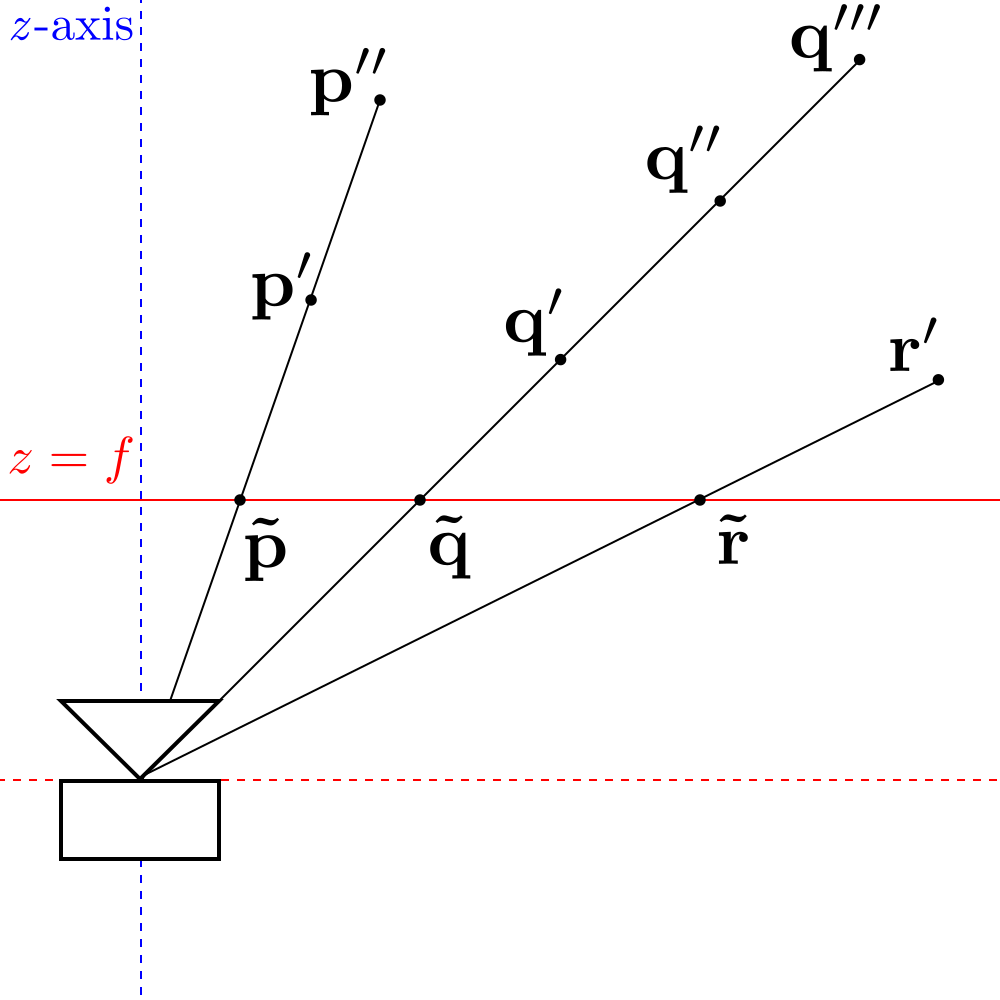
\includegraphics[scale=0.25]{Camera}
	\caption{Pinhole Camera model}
\end{figure}\newline
The location of $\mathbf{\tilde{y}}$ is determined by utilizing the \textit{similarity of triangles} between $\mathbf{x}$ and $\mathbf{\tilde{y}}$. Specifically, we see that $y_1/f=x_1/x_3$ and $y_2/f=x_2/x_3$ lets us exprss the \textit{image coordinate} $\mathbf{\tilde{y}}$ as $y_1=f\cdot x_1/x_3$ and $y_2=f\cdot x_2/x_3$. The point in the \textit{image plane} of $\mathbf{\tilde{y}}$ is derived from the point $\mathbf{x}$ in \textit{camera space} by means of the the \textit{Camera Projection Matrix} $\mathbf{P}$ such that

\begin{equation*}
\begin{split}
\mathbf{P}\cdot\mathbf{\tilde{x}}&=
\begin{bmatrix}
f & 0 & 0 & 0\\
0 & f & 0 & 0\\
0 & 0 & 1 & 0\\
\end{bmatrix}\begin{bmatrix}x_1\\x_2\\x_3\\1\\\end{bmatrix}
=\begin{bmatrix}
f\cdot x_1\\
f\cdot x_2\\
x_3
\end{bmatrix}\\
&=
x_3\cdot\begin{bmatrix}
f\cdot x_1/x_3\\
f\cdot x_2/x_3\\
1\\
\end{bmatrix}
=x_3\cdot\mathbf{\tilde{y}}
\end{split}
\end{equation*} 

This results in points $\mathbf{\tilde{x}}$ containing infinitley large values of $x_3$ being mapped to the same point $\mathbf{\tilde{y}}$ in the \textit{image plane}. This point $\mathbf{y}=0$ is referred to as the $\textit{principal point}$ in the \textit{image plane}. This assumes the \textit{principal point} is always located in the \textit{image plane} at $\mathbf{y}=0$. Projecting point $\mathbf{\tilde{x}}$ to the \textit{image plane} with arbitrary \textit{principal point} $\mathbf{p}=[p_x,p_y]^\intercal$ requires modifying the \textit{projection matrix} to include \textit{camera-specific} parameters. The \textit{camera calibration matrix} $\mathbf{K}$ is given as
\begin{equation*}
\begin{split}
\mathbf{P}\cdot\mathbf{\tilde{x}}&=
\begin{bmatrix}
f & 0 & p_x & 0\\
0 & f & p_y & 0\\
0 & 0 & 1 & 0\\
\end{bmatrix}\begin{bmatrix}x_1\\x_2\\x_3\\1\\\end{bmatrix}
=\begin{bmatrix}
f\cdot x_1+p_x\cdot x_3\\
f\cdot x_2+p_y\cdot x_3\\
x_3
\end{bmatrix}\\
&=
x_3\cdot\begin{bmatrix}
f\cdot x_1/x_3+p_x\\
f\cdot x_2/x_3+p_y\\
1\\
\end{bmatrix}
=x_3\cdot\mathbf{\tilde{y}}
\end{split}
\end{equation*} 


\section{Essential Matrix}

\par When coordinates from a reference frame are expressed as \textit{normalized image coordinates} the range of possible NIC values in the corresponding image are given by the 

%Longuet-Higgins' Fundamental Matix ~\cite{Longuet-Higgins}
\chapter{Point Interpolation}
\par
Pixels from image \textit{a} and image \textit{b} can be used to create a new images. This is done by interpolating the pixel positions ($\mathbf{p}^{a}_{uv}$ and $\mathbf{p}^{b}_{uv}$) of corresponding points between frames. Because not all pixels are established as corresponding points, pixel correspondances \textit{between} corresponding points ($\mathbf{p}_{uv}$) are calculated through bi-linear interpolation of 4 established corresponding points: 
\begin{equation*}
\mathbf{P}_{uv} = 
\mathbf{P}_{00}\cdot (1-u)\cdot (1-v)+\mathbf{P}_{10}\cdot u \cdot (1-v)+
\mathbf{P}_{01}\cdot (1-u)\cdot v +\mathbf{P}_{11}\cdot u \cdot v
\end{equation*}
This is done through the following series of linear equations
%textit{uv} calculation using 
\begin{equation*}\begin{split}
x_{uv} &= 
\begin{bmatrix}u & 1\end{bmatrix}
\begin{bmatrix}-1 & 1\\ 1 & 0\\\end{bmatrix}
\begin{bmatrix}x_{00} & x_{01} \\ x_{10} & x_{11}\\\end{bmatrix}
\begin{bmatrix}-1 & 1\\ 1 & 0\\\end{bmatrix}
\begin{bmatrix}v \\ 1\\\end{bmatrix}\\
y_{uv} &= 
\begin{bmatrix}u & 1\end{bmatrix}
\begin{bmatrix}-1 & 1\\ 1 & 0\\\end{bmatrix}
\begin{bmatrix}y_{00} & y_{01} \\ y_{10} & y_{11}\\\end{bmatrix}
\begin{bmatrix}-1 & 1\\ 1 & 0\\\end{bmatrix}
\begin{bmatrix}v \\ 1\\\end{bmatrix}\\
\end{split}\end{equation*}
or as a single matrix equation of 
\begin{equation*}
\begin{split}
\begin{bmatrix}x_{uv} & 0 \\ 0 & y_{uv}\\\end{bmatrix}
&=
\begin{bmatrix}\mathbf{u} & \mathbf{0} \\ \mathbf{0} & \mathbf{u} \end{bmatrix}^{T}
\begin{bmatrix}\mathbf{M} & \mathbf{0} \\ \mathbf{0} & \mathbf{M} \end{bmatrix}^{T}
\begin{bmatrix}\mathbf{X} & \mathbf{0} \\ \mathbf{0} & \mathbf{Y} \end{bmatrix}
\begin{bmatrix}\mathbf{M} & \mathbf{0} \\ \mathbf{0} & \mathbf{M} \end{bmatrix}
\begin{bmatrix}\mathbf{v} & \mathbf{0} \\ \mathbf{0} & \mathbf{v} \end{bmatrix}
\end{split}
\end{equation*}
where
\begin{equation*}
\begin{split}
%
\mathbf{u} =\begin{bmatrix}u \\ 1\\\end{bmatrix}
\text{, }
%
\mathbf{v} =\begin{bmatrix}v \\ 1\\\end{bmatrix}
\text{, }
%
\mathbf{X} =\begin{bmatrix}x_{00} & x_{01} \\ x_{10} & x_{11}\\\end{bmatrix}
\text{, }
%
\mathbf{Y} =\begin{bmatrix}y_{00} & y_{01} \\ y_{10} & y_{11}\\\end{bmatrix}
\text{, and }
%
\mathbf{M} =\begin{bmatrix}-1 & 1 \\ 1 & 0\\\end{bmatrix}
\end{split}
\end{equation*}
\begin{figure}[htbp]
	\centering
%	\includesvg{BiLinear_Point_Correspondance_v1}
	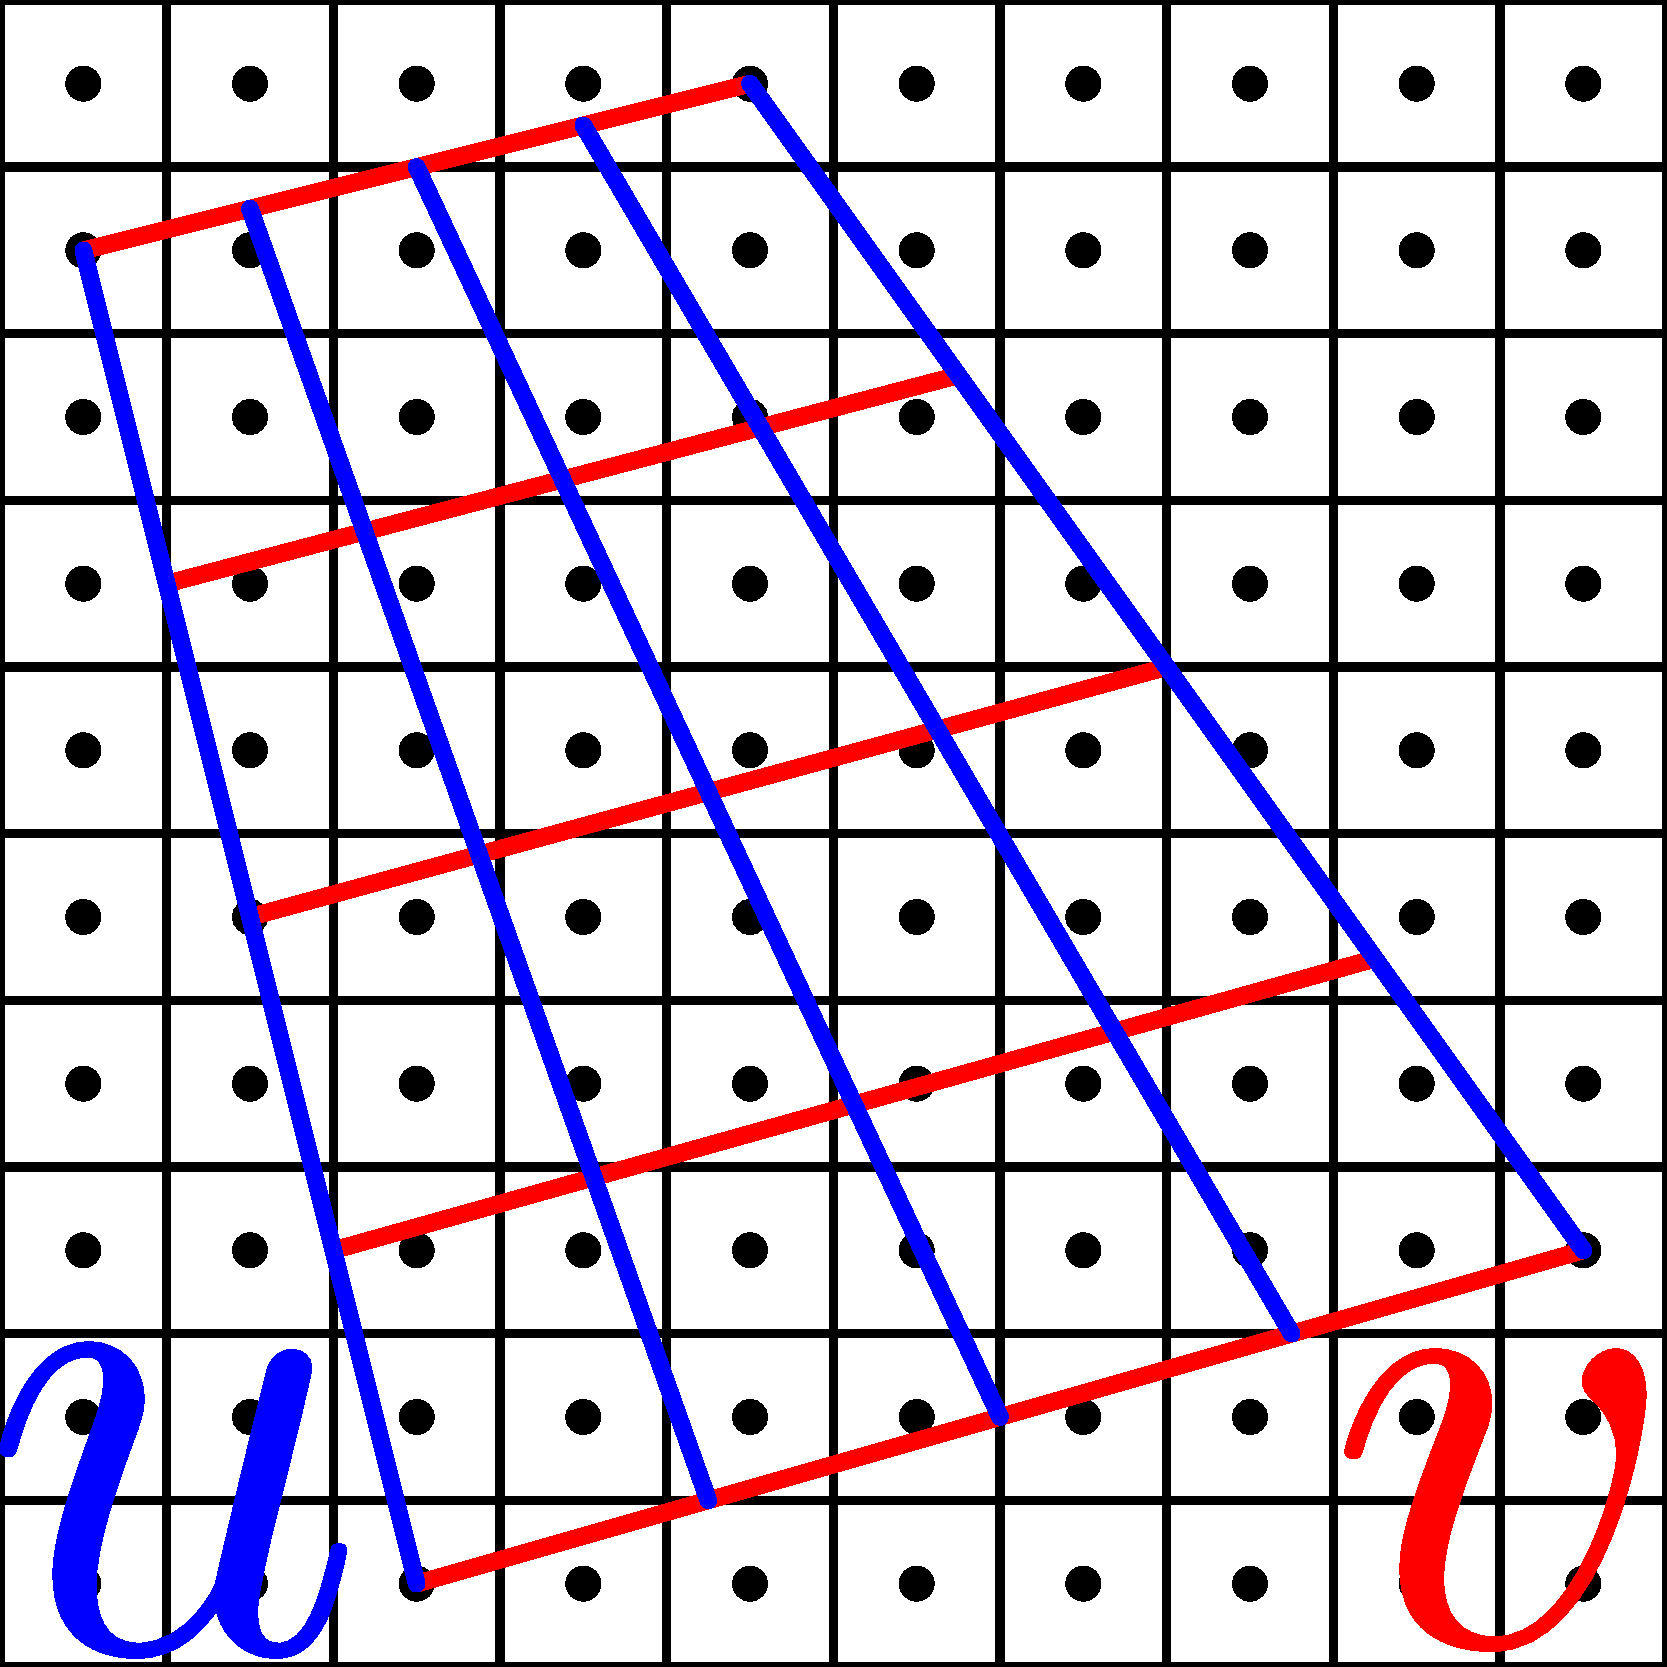
\includegraphics[scale=0.25]{BiLinear_Point_Correspondance_v1}
	\caption{Bi-Linear Point Correspondance}
\end{figure}

\chapter{Image segmentation}
\par Central to our need to localize corresponding points in stereo images is the ability to partition images by similar texture or planar attributes compared to the image at hole. Such techniques are referred to as \textit{image segmentation}. 
\par Image segmentation of regions of similar color or textures region is often approached from a graph-theory standpoint, in which individual pixels form the nodes of the graph. Edges are formed by a number of methods, the simplest of which is for each pixel to have 4 equally weighted edges connecting with the 4 immediate adjoining pixels in \textit{North}, \textit{East}, \textit{South} and \textit{West} vicinities (referred to as the \textbf{4-neighborhood region}). A common variation of this is to \textit{also} include the next 4 closest adjoining pixels in the \textit{Northeast}, \textit{Southeast}, \textit{Southwest} and \textit{Northwest} vicinities (referred to as the \textbf{8-neighborhood region}). More sophisticated methods assign edge weightings proportional to the difference in color values (\textit{scalar gray values} or \textit{euclidean distance of color vectors}) between each pixel-pair.


Binary segmentation (partitioning into two regions) can be accomplished through
min-cut / max-flow algorithms	
\chapter{Process}
The system in question contains 3 main components
\begin{enumerate}
	\item Image Acquisition System
	\begin{itemize}
		\item Webcam / Kinect set-up
		\item If Webcam should also contain Image-Processing module for:
		\begin{itemize}
			\item Feature Identification
			\item Point-correspondance
			\item Sub-Pixel interpolation
		\end{itemize}
	\end{itemize}
	\item Point Cloud Processing
	\begin{itemize}
		\item Should take inputs
		\item Should produce point-clouds as one of the output
		\item (Possible) Options for Surface Reconstruction include:
		\begin{itemize}
			\item Calculation of surface Normal through PCA
			\item Mesh construction through Delaunay trianglulation
			\item Parametrization of Bezier surface through linear-least squares.
		\end{itemize}

	\end{itemize}

\end{enumerate}

\begin{equation*}
%\cAij{i}{j}
\end{equation*}


%\bibliography{citations}{}
%\bibliographystyle{plain}


\end{document}
